%%
%% Automatically generated file from DocOnce source
%% (https://github.com/hplgit/doconce/)
%%
%%


%-------------------- begin preamble ----------------------

\documentclass[%
oneside,                 % oneside: electronic viewing, twoside: printing
final,                   % draft: marks overfull hboxes, figures with paths
10pt]{article}

\listfiles               %  print all files needed to compile this document


\usepackage[totoc]{idxlayout}   % for index in the toc
\usepackage[nottoc]{tocbibind}  % for references/bibliography in the toc

\usepackage{relsize,makeidx,color,setspace,amsmath,amsfonts,amssymb}
\usepackage[table]{xcolor}
\usepackage{bm,ltablex,microtype}
\usepackage{comment} 
\usepackage[pdftex]{graphicx}

\usepackage{fancyvrb} % packages needed for verbatim environments

\usepackage[T1]{fontenc}
%\usepackage[latin1]{inputenc}
\usepackage{ucs}
\usepackage[utf8x]{inputenc}

\usepackage{lmodern}         % Latin Modern fonts derived from Computer Modern


\usepackage{pgfplotstable, booktabs}

\pgfplotstableset{
    every head row/.style={before row=\toprule,after row=\midrule},
    every last row/.style={after row=\bottomrule}
}





% Hyperlinks in PDF:
\definecolor{linkcolor}{rgb}{0,0,0.4}
\usepackage{hyperref}
\hypersetup{
    breaklinks=true,
    colorlinks=true,
    linkcolor=linkcolor,
    urlcolor=linkcolor,
    citecolor=black,
    filecolor=black,
    %filecolor=blue,
    pdfmenubar=true,
    pdftoolbar=true,
    bookmarksdepth=3   % Uncomment (and tweak) for PDF bookmarks with more levels than the TOC
    }
%\hyperbaseurl{}   % hyperlinks are relative to this root

\setcounter{tocdepth}{2}  % levels in table of contents

% --- fancyhdr package for fancy headers ---
\usepackage{fancyhdr}
\fancyhf{} % sets both header and footer to nothing
\renewcommand{\headrulewidth}{0pt}
\fancyfoot[LE,RO]{\thepage}
% Ensure copyright on titlepage (article style) and chapter pages (book style)
\fancypagestyle{plain}{
  \fancyhf{}
  \fancyfoot[C]{{\footnotesize \copyright\ 1999-2018, "Computational Physics I FYS3150/FYS4150":"http://www.uio.no/studier/emner/matnat/fys/FYS3150/index-eng.html". Released under CC Attribution-NonCommercial 4.0 license}}
%  \renewcommand{\footrulewidth}{0mm}
  \renewcommand{\headrulewidth}{0mm}
}
% Ensure copyright on titlepages with \thispagestyle{empty}
\fancypagestyle{empty}{
  \fancyhf{}
  \fancyfoot[C]{{ }}
  \renewcommand{\footrulewidth}{0mm}
  \renewcommand{\headrulewidth}{0mm}
}

\pagestyle{fancy}


% prevent orhpans and widows
\clubpenalty = 10000
\widowpenalty = 10000

% --- end of standard preamble for documents ---


% insert custom LaTeX commands...

\raggedbottom
\makeindex
\usepackage[totoc]{idxlayout}   % for index in the toc
\usepackage[nottoc]{tocbibind}  % for references/bibliography in the toc
\usepackage{listings}
\usepackage[normalem]{ulem} 	%for tables
\useunder{\uline}{\ul}{}
\usepackage{hyperref}
\usepackage[section]{placeins} %force figs in section

\usepackage{natbib}


%-------------------- end preamble ----------------------

\begin{document}

% matching end for #ifdef PREAMBLE

\newcommand{\exercisesection}[1]{\subsection*{#1}}


% ------------------- main content ----------------------



% ----------------- title -------------------------

\thispagestyle{empty}

\begin{center}
{\LARGE\bf
\begin{spacing}{1.25}
Numerically solving the heat equation using finite-difference methods
\end{spacing}
}
\end{center}

% ----------------- author(s) -------------------------

\begin{center}
{\bf Johan Nereng}
\end{center}

    \begin{center}
% List of all institutions:
\centerline{{\small Department of Physics, University of Oslo, Norway}}
\end{center}
    
% ----------------- end author(s) -------------------------

% --- begin date ---
\begin{center}
Des 14, 2018
\end{center}
% --- end date ---

\vspace{5cm}
\begin{abstract}
This project aims to examine the suitability of three finite-difference methods in numerically approximating the heat equation; the explicit forward Euler scheme (FW), the implicit backward Euler scheme (BW), and the Crank-Nicolson scheme (CN). By comparing the results produced by these methods to the closed form solution of a simplified heat diffusion problem, this project finds that the Crank-Nicolson scheme (local truncation error $\sim O((\Delta t)^2)$ and $O((\Delta x)^2)$) is concluded as the overall most precise method due to relative errors $\sim (\Delta x)^2$. The two other schemes are determined unsuitable for certain types of solutions. In the case of FW, solutions at a time, $T$, with a high ratio to the characteristic diffusion time ($T\sim T_*$) and discretization points $\sim 10^2$. In the case of BW, solutions at $T<<T_*$. Additionally, this project makes a cursory examination of the application of FW to a diffusive problem in two spatial dimensions, where the only certain conclusion was the the scheme produced results similar in shape and magnitude to the closed form solution.
\end{abstract}

\newpage
\textit{\textbf{Authors' comment:} During this project, I have spent a great amount of time both reading on PDEs and debugging code. Reading up on PDEs was rewarding and I enthusiastically spent too much time on it with regards to the extensive difficulties I encountered in implementing the approximation methods, and seeing how I've neglected preparing for an upcoming exam in abother subject. This has led me to re-learn a lesson which I've forgotten many times: the value of writing down a work plan when starting on a large project. This was further underlined when I suddenly realized that I the deadline was closing in, and I had spent too much time on reading, and way too much time on examining details related to managing data flow - such as establishing a more organized system of directories, and trying out Latex and Python packages. Lastly, I've learned a lot about debugging - especially from implementing the 2D case, where I wasted hours upon hours searching in an unsystematic way for an error that I easily found after half an hour of sleep and going through the program line by line, jumping in and out of functions and files. }
\section{Introduction}
When a system is in a state where the spatial density distribution of some quantity is unequilibrated, a flow from regions of high density to regions of low density occurs. This phenomenon, known as diffusion, is described by Fick's first law, named after the German physician Adolf Eugen Fick. Fick's first law states that the diffusional flux \footnote{The diffusional flux is the quantity transport per unit time per unit area, perpendicular to the direction of the diffusion} is proportional to the concentration gradient of the diffusing component \citep[pp. 339-340]{MatSci}. Less precisely, it can be said that the strength of the diffusional flow at a specific place, corresponds to how strongly the density varies around that place. Application of a conservation law appropriate to the diffusing quantity leads to what is either known as Fick's second law, or the continuity equation \citep[pp.341-342]{MatSci}). \\
The continuity equation, may, under the constraints of linearity between gradient and flow, be expressed as the partial differential equation (PDE) known as the heat equation. Diffusion problems where one can assume such linearity may be expressed through \eqref{eq:HeateqGEN}. Typically, such linearity is the domain of bodies with uniform properties. Along with the appropriate initial conditions (ICs) and boundary conditions (BCs), the closed form solution of the PDE may sometimes be obtained using certain methods, of which some are outlined later in this project. However, when describing real physical systems, such closed form solution are often not obtainable, yet the same computational procedures may often be applied in providing a numerical solution. Finite-difference methods (FDM) are perhaps the most commonly applied type of method for solving PDEs. In short, FDMs are discretization methods in which the derivatives of a differential equation is approximated using by finite differences \citep[p. 46]{compPDE}, usually obtained through a Taylor expansion. 

\paragraph{Project flow:} This project starts by introducing the heat equation problem and a simple example to which it may be applied - the equalization of heat in a one dimensional rod. Then, a procedure for scaling the heat equation is outlined, and applied to the PDE obtained from the rod problem. A general approach to discretizing a scaled heat equation problem is thereafter presented, before the finite Finite-difference methods used in the project are described mathematically.\newline
The explicit forward Euler scheme, the implicit backward Euler scheme, and the Crank-Nicolson schemes are brought to the form of matrix products, which in the case of the two latter FDMs are then used to procure scheme algorithms. As the Crank-Nicolson scheme may be expressed as a combination of the two Euler schemes, setting up it's algorithm depends on linking it's mathematical expression to that of the two Euler methods. This is done through the matrix representations. The nature of the explicit forward Euler scheme is such that it may be expressed rather straight forward from a mathematical description to an algorithm - it's matrix product is solely used to connect it to the Crank-Nicolson scheme. In contrast to the other two methods, the explicit forward Euler scheme is not always stable. It's stability relies on the ratio between the time step,$\Delta t$, and the square of step in spatial coordinates, $(\Delta x)^2$. Due to this, the algorithms use the explicit forward Euler methods stability criteria when choosing $\Delta t$ \newline
Having expressed the algorithm for each method, the project goes on to implementing the algorithms in a single program, using the scaled rod PDE. The program is then tested with emphasis on relative error, compared with the closed form solution. A procedure for finding the CFS is described in a section of it's own. \newline
Lastly, the heat equation is extended to two spatial dimensions. Here, the explicit forward Euler scheme is utilized, albeit in a more extensive form, as it now aims to solve for one more variable. The mathematical expression for this method in 2 (spatial) dimensions is then brought to the form of an algorithm, which is implemented into a new program. The results produced by this program is then compared with the CFS to the 2D heat equation, which is outlined in a section of it's own - though with less detail than the 1D case. In comparing the approximation method with the CFS, attention is especially given to the stability of the solution as a function of constraints on the $\Delta t$ and $h=\Delta x =\Delta y$.

\paragraph{Main findings}
Through examining the solutions produced by the algorithm implementations, this project goes on to concluding that overall error magnitudes are $\sim (\Delta x)^2$ and to a varying degree  $\sim \Delta t (\Delta x)^2$. Furthermore, the Crank-Nicolson scheme (local truncation error $\sim O((\Delta t)^2)$ and $O((\Delta x)^2)$) is concluded as the overall most precise method due to relative errors $\sim (\Delta x)^2$.  The two other schemes are determined unsuitable for some types of solution. In particular, the implicit backward Euler scheme is concluded unsuited for solution that with few time iterations (diffusion time $<\sim 0.1$ characteristic diffusion time), due relative errors one order of magnitude larger than the Crank-Nicolson method. The explicit forward Euler method is concluded as unsuited in the opposite case, where the solution is procured after a large number of iterations (diffusion time $>\sim 0.1$ characteristic diffusion time), and the number of spatial discretization points are large ($\sim 10^2$). \newline
In the case of two spatial dimensions, this project finds that the explicit forward Euler produces solutions similar in shape and order of magnitude to the the closed form solution. In the two dimensional case, no further conclusions are drawn, due to results which indicate an uncharacteristic independence on $h$. 
\paragraph{Tools used:} 
In constructing the code, $C++$ with the armadillo library was used. More on this under \hyperref[M.AlgoImpl]{algorithm implementation}. Python, with the matplotlib and numpy library, was utilized in procuring plots and processing the data output from the solver. In addition, a number of books and websites were drawn upon to build the theoretical basis for the project described in the methods section. These are listed at the end of project. All programs, results and files used in this project may be found on the author's \href{https://github.com/johanere/CP5}{Github repository}




\section{Methods}
\subsection{The Heat Equation}
\label{M.1DHQ}
The heat equation \eqref{eq:HeateqGEN}, also known as the diffusion equation, is a special case of the continuity equation in which the relationship between flow and density gradient is linear \citep{HJ15}. A wide range of diffusion problems may, with sufficient simplifications, be expressed through this equation, and solved provided suitable ICs and BCs. These ICs represent the state of the system, or the distribution of the diffusive quantity , at $t=0$, while the BCs apply restrictions on the diffusion on the periphery of body in which the diffusion takes place.\newline
\begin{equation}
\frac{\partial u}{\partial t}=D \nabla^2 u
\label{eq:HeateqGEN}
\end{equation}
\textit{Where $u$ signifies the density of the diffusive quantity, $t$ the time, while $D=constant$ is a proportionality constant -  also known as the diffusion constant. } \newline

As an example of the application of the heat equation, consider a one dimensional system consisting of a rod of length $L$, with each end of the rod in contact with a thermal bath.  If $x$ denotes the spatial coordinates along the length of the rod, the thermal gradient, $u=u(x,t)$, is subject to heat diffusion unless equilibrated. Assume that the two thermal baths each hold one end of the rod at constant temperature; $u_0$ (at $x=0$) and $u_1=u_0 +\Delta u, \quad \Delta u>0$ (at $x=L$), where $\Delta u$ is the difference in temperature between the two heat baths. This means that the BCs are:
\begin{align}
u(0,t)=u_0, \quad t \geq 0 \\
u(L,t)=u_1, \quad t \geq 0
\end{align}
Furthermore, assume that the rod has thermally equilibrated with the heat bath holding temperature $u_0$ before $x=L$ is put into contact with the other thermal bath at $t=0$. Thus the ICs are:
\begin{equation}
u(x,0)=f(x)=  \begin{cases}
 & u_0, \quad 0\leq x < L\\
 & u_1, \quad x=l
  \end{cases}
\end{equation}

Lastly, the rod has the following uniform properties; thermal conductivity, $\kappa(W/(m\cdot K)$, specific heat capacity $c(J/(kg \cdot K))$, and (mass) density $\rho(kg/m^3)$, the diffusion constant $D$ may be expressed as $D=\frac{\kappa}{c \rho}$ \citep[p.304]{HJ15}. Assuming linear diffusion, the time evolution of heat distribution in the rod may then be expressed in terms of the heat equation \eqref{M.1DHQ}, which results in the following mathematical problem:

\begin{align}
PDE:&\quad \frac{\kappa}{c \rho}\frac{\partial^2 u(x,t)}{\partial x^2}=\frac{\partial u(x,t)}{\partial t} \label{eq:rod}\\
ICs:&\quad u(x,0)=f(x)=  \begin{cases}
  u_0, \quad 0\leq x < L\\
 u_1, \quad x=L
  \end{cases} \label{eq:rodIC}\\\
BCs:& \quad u(0,t)=u_0, \quad t \geq 0 \quad u(L,t)=T_1, \quad t \geq 0 \label{eq:rodBC}
\end{align}


\subsection{Scaling the Heat Equation}
Both the algorithms developed later in this project and the outlined method for obtaining a CFS, assumes a scaled diffusive problem. Scaling often requires considerable insight in the problem, on account of choosing suitable characteristic variables. The following outlined scaling procedures are from an MIT course on PDEs, and does not go into detail on choice of characteristic variables - the choice of which is left open (for more details see \cite{Hancock}). Below, heat is referred to the diffusive quantity, $u$. The procedure does however apply to other diffusive quantities involved in diffusion problems applicable to the heat/diffusion equation. \newline

First, dimensionless variables are introduced:
\begin{align}
\hat{x}=\frac{x}{L_*}, \qquad \hat{t}=\frac{t}{T_*}, \qquad \hat{u}(\hat{x},\hat{t})=\frac{u(x,t)}{U_*},  \qquad\hat{f}(\hat{x}) =\frac{f(x)}{U_x}
\end{align}
Where $[L_*]=L$, $[T_*]=T$, $[U_*]=U$ are characteristic length, time and temperature. Using the chain rule yields:
\begin{align*}
u_t=\frac{\partial u}{\partial t}=U_* \frac{\partial \hat{u}}{\partial \hat{t}}\frac{\partial \hat{t}}{\partial t}=\frac{U_*}{T_*}\frac{\partial \hat{u}}{\partial \hat{t}} 
\end{align*}
And similarly:
\begin{align*}
u_x=\frac{U_*}{L_*}\frac{\partial \hat{u}}{\hat{x}} \\
u_{xx}=\frac{U_*}{L_*^2}\frac{\partial^2 \hat{u}}{\hat{x}^2} \\
\end{align*}
Substitution into the heat equation \eqref{eq:HeateqGEN}:
\begin{align*}
u_t=D u_{xx} \quad \rightarrow \quad \frac{\partial \hat{u}}{\partial \hat{t}}= D \frac{T_*}{L_*}\frac{\partial^2 \hat{ u}}{\partial \hat{x}^2}
\end{align*}
Then, setting $T_*=L_*^2/D$ results in: 
\begin{align}
\frac{\partial \hat{u}}{\partial \hat t}=\frac{\partial^2 \hat{u}}{\partial \hat{x}^2} \label{eq:1dscaled}
\end{align}
\eqref{eq:1dscaled} now holds the scaled heat equation problem. All that is left is to similarly scale the ICs and BCs pertaining to the particular problem at hand.

\paragraph{Applying scaling:} The scaling procedures above are now applied to the case of the one dimensional rod problem from the section \hyperref[M.1DHQ]{on the heat equation} - in the future simply referred to as the rod problem. The characteristic length of the problem is taken to be the length of the rod, so $L_*=L$. With the restrictions posed on the rod, $u_0$ ($u_0<u_1$) is the lowest temperature that any part of the rod may have, therefore $u_0$ is defined as $u=0$. This makes the the difference in temperature of the two thermal bath a natural choice for characteristic temperature, that is; $U_*=\Delta u$. Lastly, characteristic time is set to $T_*=L_*^2/D=L^2 \frac{\kappa}{c \rho}$. Renaming $\hat{u}$ as $u$, $\hat{t}$ as $t$ , and so on, then yields the following scaled diffusion problem:

\begin{align}
PDE:&\quad \frac{\partial^2 u(x,t)}{\partial x^2}=\frac{\partial u(x,t)}{\partial t} \label{eq:scaled.rod}\\
ICs:&\quad u(x,0)=f(x)=  \begin{cases}
  0, \quad 0 < x < 1\\
 1, \quad x=1
  \end{cases} \label{eq:scaled.rodIC}\\\
BCs:& \quad u(0,t)=0, \quad t \geq 0 \quad u(1,t)=1, \quad t \geq 0 \label{eq:scaled.rodBC}
\end{align}

\subsection{Approximation methods}
\label{M.ApproxMethods}
The approximation methods used in this project are the explicit forward Euler, the implicit Backward Euler, and the Crank-Nicolson scheme with a time-centered scheme. All of these three methods are FDMs, which means that they approximate derivatives  by using a sum of differences, where the terms in this case are obtained from Taylor series expansions of the function to be differentiated. The description of the methods in this project is restricted to the expressions involved in the scaled heat equation \eqref{eq:Approxim.heateq}, however application to other types of PDEs are readily available in literature such as the book by A. Tveito and R.Winther on PDEs in numerical computations \cite{compPDE}.
\begin{align}
PDE:& \quad \frac{\partial^2 u(x,t)}{\partial x^2}=\frac{\partial u(x,t)}{\partial t} \label{eq:Approxim.heateq}\\
ICs:& \quad u(x,0)=f(x), \quad 0< x < 1 \label{eq:Approxim.IC}\\
BCs:& \quad u(0,t)=a, \quad t \geq 0, \quad u(1,t)=b, \quad t \geq 0  \label{eq:Approxim.BC}
\end{align}

In order to apply the notation pertaining to discrete variables when describing the methods, the discretization of relevant variables is now outlined, assuming that the problem has been properly scaled. The spacial domain, $x \in [0,1]$, is discretized over $n+1$ grid points, such that $x_i=i \Delta x$, $i=0,1,...,n+1$, where $\Delta x= \frac{1}{n+1}$. Similarly, $t=[0,1]$, is is expressed as $t_j=j \Delta t$, $j\geq 0$. The dizcrete approximation of the diffusing quantity, $u \in [0,1]$ is then defined as $u(x_i,t_j)=u_{i,j}$, and the discrete ICs $f(x_i)$ and BCs $u_{0,j}$ and $u_{n+1,j}$. 

\paragraph{The explicit forward Euler scheme} uses a forward Taylor expansion of the first order for the time derivative. That is\citep[p. 305]{HJ15}:
\begin{equation}
u_{t} \approx \frac{u(x, t +\Delta t)- u(x,t)}{\Delta t} =\frac{u(x_i, t_{j+1})- u(x_i,t_j)}{\Delta t} =\frac{u_{i,j+1}- u_{i,j}}{\Delta t} \label{FWD1d.ut}
\end{equation}
Being a first order approximation, the local trunction error (LTE) of this approximation is $O(\Delta t)$. The spatial derivative, in this case $u_{xx}$, is approximated using a second order Taylor series expansion around $u_{i,j}$:
\begin{align}
u_{xx} \approx \frac{u_{i+1,j} -2u_{i,j}+u_{i-1,j}}{\Delta x^2} \label{FWD1d.uxx}
\end{align}
In contract to the approximation of $u_t$, $u_{xx}$ is a second order approximation which yields an LTE of $O((\Delta x)^2)$. Substituting \eqref{FWD1d.ut} and \eqref{FWD1d.uxx} into \eqref{eq:Approxim.heateq}:
\begin{align*}
\frac{u_{i+1,j} -2u_{i,j}+u_{i-1,j}}{(\Delta x)^2}=\frac{u_{i,j+1}- u_{i,j}}{\Delta t} 
\end{align*}
Defining $\alpha=\Delta t/(\Delta x)^2$ and solving for $u(x,t+\Delta t)=u_{i,j+1}$:
\begin{align}
u_{i,j+1}= \alpha u_{i-1,j}+(1-\alpha)u_{i,j}+\alpha u_{i,j} \label{eq:Approximation.FWDnew}
\end{align}

Specifying $\Delta x$ and $\Delta t$, and setting $j=0$, the left hand side of \eqref{eq:Approximation.FWDnew} is known through $f(x_i)$ \eqref{eq:Approxim.IC}, the ICs of the PDE. This in turns enables iteratively solving explicitly for $u_{j,i+1}$, which is the basis for the later described explicit forward Euler algorithm. In order to express the Crank-Nikcolson scheme (CN) effectively, \eqref{eq:Approximation.FWDnew} is now brought to matrix form - more on the CN scheme later.  \newline
Recalling that the BCs, $u_{0,j}$ and $u_{1,j}$, are the constants $a$ and $b$ (Dirichlet BCs), and if $a=b=0$, then the solution at $t=j \Delta t$, that is $u_{i,j}$, may be expressed by the vector:
\begin{equation} 
V_j=
\begin{bmatrix}
v_{1,j} \\ v_{2,j} \\ ...\\ v_{n,j}
\end{bmatrix}
\end{equation}
If $a$ and/or $b$ however are not equal to zero, $V_j$ is not a valid expression for $u_{i,j}$ as it is missing $u_{0,j}$ and $u_{n+1,j}$. This may be addressed by determining the (discretized) steady-state of the diffusive problem, $\tilde{u}_{i,j}$, and making the substitution $u_{x_i,t_j}=v_{x_i,t_j}+\tilde{u}_{i,j} \implies v_{x_i,t_j}=u_{x_i,t_j}-\tilde{u}_{i,j}$ such that the BCs of $v(x_i,t_j)$, $\tilde{a}=\tilde{b}=0$. More on this under the section on \hyperref[M.CFS1d]{closed form solutions to the 1D heat equation}, where $\tilde{u}_{i,j}$ is referred to as $u_E$. Solving for $v_{i,j}$ in a similar fashion as $u_{i,j}$ in the $a=b=0$ case, then later substituting back, a PDE with inhomogeneous BCs may also be expressed through the vectors $V_j$, though this requires that the ICs are shifted to $\tilde{f}(x_i)=-\tilde{u}_{i,j}$.\newline
Having expressed $u_{i,j}$ through the vector $V_j$, \eqref{eq:Approximation.FWDnew} corresponds to the following matrix product:
\begin{equation}
V_{j+1}=\mathbf{A}V_j
\end{equation}
In which $\textbf{A}=  \begin{bmatrix}
                           1-2\alpha & \alpha & 0 &\dots   & \dots &0 \\
                           \alpha & 1-2\alpha  &  \alpha &0 &\dots &\dots \\
                           & \dots   & \dots &\alpha   &1-2\alpha& \alpha \\
                      
                           0&\dots    &  & 0  &\alpha & 1-2\alpha \\
              			\end{bmatrix}$ 
\newline
              			
\paragraph{The implicit backward Euler scheme}  is an alternative method to the explicit Forward scheme. Instead of using forward  approximation to $u_{t}$, this implicit scheme uses a first order backward approximation \citep[308]{HJ15}:

\begin{equation}
u_{t} \approx \frac{u_{i,j}- u_{i,j-1}}{\Delta t} \label{BW.ut}
\end{equation}
As with the forward case, this first order approximation has an LTE $O(\Delta t)$. In combination with the already described second order approximation \eqref{FWD1d.uxx}, and $\alpha=\Delta t/\Delta  x^2$, which yields:
\begin{equation}
u_{i,j-1}=-\alpha u_{i-1,j}+(1-\alpha)u_{i,j}-\alpha u_{i+1,j} \label{eq:BWuxx}
\end{equation}
Applying the same procedures described for the explicit method with respect to BCs and ICs, the vector $V_{j}$ is again defined, such that \eqref{eq:BWuxx} may be written as the matrix product:
$V_{j-1}=BV_j$,\\
where
$\textbf{B}=  \begin{bmatrix}
                           1+2\alpha & -\alpha & 0 &\dots   & \dots &0 \\
                           -\alpha & 1+2\alpha  &  -\alpha &0 &\dots &\dots \\
                           & \dots   & \dots &\dots   &1+2\alpha & -\alpha \\
                      
                           0&\dots    &  & 0  &-\alpha & 1+2\alpha \\
              			\end{bmatrix}$ 


This $n \times n$ matrix product may solved by for example LU decomposition, which takes $\sim O(n^3)$ floating point operations \citep[173]{HJ15}. However, since \textbf{B} is a sparse matrix (most elements are equal to zero), such rigorous methods are overly complicated. $B$ is a tridiagonal matrix, and as such, may be solved for $V_j$ through tridiagonal matrix methods, resulting in fewer floating point operations ($\sim O(n)$). Drawing on the methods described in project 1 \cite{P1}, the matrix equation $V_{j-1}=BV_j$, may be reduced to: \newline
$\begin{bmatrix} \tilde{v}_{1,j-1} \\ \tilde{v}_{2,j-1}\\ \cdots \\ \cdots \\ \tilde{v}_{n,j-1}\end{bmatrix}=\tilde{V}_{j-1}=\tilde{B}V_j$, with

\[
    \mathbf{\tilde{B}} = \begin{bmatrix}
                      \tilde{d_1}& -\alpha & 0 &\dots   & \dots &\dots  \\
                           0 & \tilde{d_2} & -\alpha &\dots &\dots &\dots \\
                           & 0 & d_3 & -\alpha & \dots & \dots     \\
                           & \dots   & \dots &\dots   &\dots  &\dots  \\
                           &   &  &0  &\tilde{d_{n-1}}& -\alpha  \\
                           &    &  &   &0 & \tilde{d_n}  \\
                      \end{bmatrix}
                      \label{finalmatrixproduct}
\]
Where \begin{equation}
\tilde{d_i} =
  \begin{cases}
                                  (1+2 \alpha)+\frac{\alpha^2}{\tilde{d}_{i-1}},  & \text{for i=2,3,...,n}\\
                                   1+2 \alpha ,  & \text{for i=1} \\

  \end{cases}
\label{eq:tilded_i}
\end{equation}
\begin{equation}
\tilde{v}_{i,j-1}=
  \begin{cases}
                                  v_{i,j-1}+\frac{\alpha \tilde{v}_{i-1,j-1} }{\tilde{d}_{i-1}}, & \text{for i=2,3,...,n}\\
                                   v_{i,j-1} ,  & \text{for i=1} \\

  \end{cases}
\label{eq:b_i}
\end{equation}

This matrix product yields the relation $v_{n,j} \tilde{d}_n=\tilde{v}_{n,j-1}$. Since $\tilde{d}_{n-1} v_{n-1,j} + c_{n-1} v_n = \tilde{v,j}_{n-1,j-1}$ and so on, $v_{i,j}$ may be backwards substituted:\par 

\begin{equation}
   v_{i,j} =
  \begin{cases}
                                  \frac{\tilde{v}_{n,j-1}}{\tilde{d}_n} ,  & \text{for i=n}\\
                \frac{\tilde{v}_{i,j-1}+\alpha v_{i-1,j}}{\tilde{d}_i}, , & \text{for i=1,2,...,n-1}                    \\

  \end{cases}
\label{eq:v_i}
\end{equation}
Which is the starting point for the explicit backward Euler algorithm presented later. 

\paragraph{The Crank-Nicolson scheme} (CN) combines the explicit and implicit methods described above through  the paramter $\theta$. The $\theta$-rule leads to the equation \cite[p.310]{HJ15}: 

\begin{equation}
\frac{\theta}{(\Delta x)^2}(u_{i-1,j}-2u_{i,j}+u_{i,j})+\frac{1-\theta}{\Delta x}(u_{i+1,j-1}-2u_{i,j-1}+u_{i-1,j-1})=\frac{1}{\Delta t}(u_{i,j}-u_{i,j-1})
\label{eq:thetarule}
\end{equation}

$\theta=0$ leads to the already described explicit forward Euler scheme, while $\theta=1$ results in the implicit backward Euler scheme. $\theta=1/2$ however, leads to the so called The Crank-Nicolson scheme \cite[p.311]{HJ15}:
\begin{equation}
-\alpha u_{i-1,j}+(2+2\alpha)u_{i,j} - \alpha u_{i+1,j}=\alpha u_{i-1,j-1}+(2-2\alpha)u_{i,j-1}+\alpha u_{i+1,j-1}
\label{eq:CN}
\end{equation}
Where $\alpha$ is as previously defined. This approximation is based on combining the time derivatives from both the explicit and the implicit scheme, meaning that the time derivative becomes a centred Taylor expansion with LTE $O(\Delta t^2)$. As the explicit and implicit scheme both use the same approximation to $u_{xx}$, the LTE for the spatial approximation remains $O((\Delta x)^2)$. \newline
The next step, yet again, requires BCs: $a=b=0$.  In the case of inhomogeneous Dirichlet BCs, apply the procedure for change of variables described under in the explicit scheme. With $a=b=0$,  \eqref{eq:CN} yields the matrix product:
\begin{equation}
(2 \mathbf{I}+\alpha \mathbf{C})V_j= (2\mathbf{I}-\alpha \mathbf{C})V_{j-1}
\end{equation}
Where $\mathbf{C} = \begin{bmatrix}
                      		2& -1 & 0 &\dots   & \dots &\dots  \\
                           -1 & 2 & -1 &0 &\dots &\dots \\
                           & \dots & \dots& \dots& \dots & \dots     \\
                           0&  \dots & \dots &-1  &2& -1  \\
                           0&  \dots  &\dots  &\dots  &-1 & 2  \\
                      \end{bmatrix}$

Reorganizing the matrix product gives:
\begin{align}
V_j=(2 \mathbf{I}+\alpha \mathbf{C})^{-1} (2\mathbf{I}-\alpha \mathbf{C})V_{j-1} \\
\end{align} 
Recalling \textbf{A} from the explicit scheme matrix representation, and \textbf{B} from the implicit scheme matrix representation, 
\begin{align}
2\mathbf{I}-\alpha \mathbf{C} = \textbf{A}+\mathbf{I}\\
2 \mathbf{I}+\alpha \mathbf{C}=\mathbf{B}-\mathbf{I}
\end{align} 
Which leads to the following sequential matrix products, for solving the Crank-Nicolson scheme:
\begin{align}
\hat{V}_{j-1}=(2\mathbf{I}-\alpha \mathbf{C})V_{j-1}= (\textbf{A}+\mathbf{I})V_{j-1} \\
(2 \mathbf{I}+\alpha \mathbf{C}) V_j=(\mathbf{B}+\mathbf{I}) V_j=\hat{V}_{j-1}
\end{align}
\subsection{Approximation errors and stability}
As mentioned in the previous section outlining the approximation methods. The forward and backward first order time derivative approximations both have a local truncation errors $\sim O(\Delta t)$. Similarly, the second order spatial derivative approximation yields and LTE $\sim O((\Delta x)^2$. As both the explicit forward Euler scheme and the implicit backward Euler scheme use these approximation, they both have LTE $O(\Delta t)$ and $O((\Delta x)^2)$. As mentioned, the Crank-Nicolson scheme however uses a time centred spatial derivative approximation with LTE $\sim O(\Delta t^2)$, derived in the lecture notes from in course Computational Physics at the University of Oslo \citep[p.311]{HJ15}. Thus, the CN scheme as LTE $O(\Delta t^2)$ and $O((\Delta x)^2)$. \newline

In terms of stability, a general method, called Von Neumann's Stability Analysis - described in detail in \citep[p.132-134]{compPDE}, may be applied in order to study the stability of both numerical and analytical solutions. Here, such analysis is only applied to problems analogous to the scaled rod problem. As will be described in more detail later, solutions to the heat equation in one dimension with homogeneous BC are on the form 
\begin{equation}
\{T_n(t) sin (n \pi x)\}_{n=1}^{n=\infty}
\end{equation}
where $T_n(t)=e^{-n^2\pi^2t}$. That is, the solution may be expressed as a family of solutions. In Von Neumann's Stability Analysis, this family of solution, along with families of solutions from  Neumann data and periodic boundary conditions are grouped together, such that the solution of either type of problem may be obtained through a linear combinations of:
\begin{equation}
F=\{T_n(t)e^{ik\pi x}\}_{n=1}^{n=\infty}
\end{equation} 
And in the case of discrete problems
\begin{equation}
F_\Delta=\{(a_n)^j e^{in\pi x_i}\}_{n=1}^{n=\infty}
\end{equation} 
Where $(a_n)^j$ is referred to as the amplification factor. Drawing on this, the stability of the three methods used in this project may be examined. Recalling the approximations in the explicit Euler scheme:
\begin{align*}
\eqref{FWD1d.ut} =& \eqref{FWD1d.uxx} \\
\frac{u_{i,j+1}- u_{i,j}}{\Delta t}=&\frac{u_{i+1,j} -2u_{i,j}+u_{i-1,j}}{(\Delta x)^2} 
\end{align*}
Substituting $u_{i,j}$ with a particular solution from $F_{\Delta x}$:
\begin{align*}
\frac{(a_n)^{j+1} e^{in\pi x_i}- (a_n)^j e^{in\pi x_i}}{\Delta t}=&\frac{(a_n)^j e^{in\pi x_{i+1}} -2(a_n)^j e^{in\pi x_i}+(a_n)^j e^{in\pi x_{i-1}}}{(\Delta x)^2} 
\end{align*}
or 
\begin{align*}
\frac{(a_n)^{j+1}- (a_n)^j }{\Delta t} e^{in\pi x_i}=&\frac{ e^{in\pi x_{i+1}} -2 e^{in\pi x_i}+ e^{in\pi x_{i-1}}}{(\Delta x)^2} (a_n)^j
\end{align*}
Dividing both sides by $(a_n)^j e^{in\pi x_{i+1}}$
\begin{align*}
\frac{(a_n)^{j}- 1 }{\Delta t} =&\frac{ e^{in\pi x_{1}} -2 + e^{in\pi x_{-1}}}{(\Delta x)^2}
\end{align*}
Since $x_i=\Delta x \cdot i$:
\begin{align*}
\frac{(a_n)^{j}- 1 }{\Delta t} =&\frac{ e^{in\pi \Delta x} -2 + e^{-in\pi \Delta x}}{(\Delta x)^2}
\end{align*}
And using $cos(x)=\frac{1}{2}\left(e^{ix}+e^{-ix} \right)$:
\begin{align*}
\frac{(a_n)^{j}- 1 }{\Delta t} =&2 \frac{cos(n\pi \Delta x)-1}{(\Delta x)^2}\\
=&-4 \frac{sin^2(n\pi \Delta x/2)}{(\Delta x)^2}
\end{align*}
Solving for $a_n$:
\begin{align}
a_n=1-4 \frac{\Delta t}{(\Delta x)^2}sin^2(n\pi \Delta x/2)
\end{align}
As $|T_n(t)|=|e^{-n^2\pi^2t}|\leq 1$ for all $n$, the same requirement is put on $|(a_n)^j|\leq 1$, which means that  
$0 \leq 4 \frac{\Delta t}{(\Delta x)^2}sin^2(n\pi \Delta x/2) \leq 1 \implies \frac{\Delta t}{(\Delta x)^2} \leq 1/2$. \newline
This means that when using the explicit forward Euler scheme, in order to obtain a stable numerical solution, $\frac{\Delta t}{(\Delta x)^2} \leq 1/2$.
Similar analysis of the two other schemes leads to the conclusion that the implicit backward Euler and the Crank-Nicolson scheme are stable for all choices of $\Delta x$ and $\Delta t$ \citep[p.312]{HJ15}.
\subsection{Algorithms}
Developing a program which may numerically solve the Heat Equation (HQ) using either of the three approximation methods requires setting up the algorithms for each methods. Each algorithm will be tested for accuracy relative to the CFS, as a function of $\Delta x$ and time evolution. In order to accomplish this while assuring that as few parameters as possible needs to be specified in each program execution, the algorithms are developed to take only $\Delta x= dx$ and the total time $T$ as initiation parameters. In addition, developing general diffusion problem algorithms which require that the PDE, ICs and BCs are scaled, secures the streamlining of parameter calculations based on initiation parameters, and their range. As such, the total time $T$, temperature $U$, and position $x$ all have a range of $[0,1]$, where where $x=0$ and $x=1=(n+1)$. In the case of $T=1$, this corresponds to equilibration of temperature, since $T=T_*$ is the characteristic time scale of the diffusive process. \newline

Recalling that $\Delta x=\frac{1}{n+1} \implies n=\frac{1}{\Delta x}-1$. Thus, using $\Delta x$ as an initiation parameter from which $n$ is defined, requires $\Delta x$ to be chosen with some care, such that $n$ becomes an integer. $\Delta t= dt$ is calculated based on the stability criteria for the explicit scheme: $dt=0.5 \cdot dx^2$. The algorithms assumes BCs $a=b=0$, if this is not the case, the initial conditions must be shifted (see section on \hyperref[M.ApproxMethods]{approximation methods}). 

\begin{center}\fbox{\parbox{\textwidth}{{\textbf{HQ: Explicit forward Euler algorithm}}
\begin{enumerate}
\item Initialize PDE
\subitem - Set $dx$ at $T$
\subitem - Define steady state $\tilde{u_i}$,  ($\tilde{u}_0=\tilde{u}_{n+1}=0$)
\subitem - Calculate $n=1/dx -1, \quad dt=0.5 \cdot dx^2$
\subitem - Calculate $\alpha=dt/dx^2, \quad \beta=1-2\alpha$
\subitem - Initiate and set:
\subitem 	$x_i= i \cdot dx \quad  v_i=-\tilde{u_i}, \quad i=0,1,2,...,n+1$
\subitem - Initiate: previous solution vectorized $u$, time $t=0$
\item Advance solution in time
\subitem - Set $u=v$ 
\subitem - $v_1=\alpha u_1+\beta u_2$
\subitem - $v_i=\alpha \left(u_{i-1}+u_{i+1}\right) +  \beta u_i,\quad i=2,...,n-1$
\subitem - $v_n=\alpha u_n+\beta u_{n-1}$
\subitem - $t=t+dt$
\item If $t<T$, repeat step 2.
\item Else end simulation.  
\end{enumerate}}}\end{center}

\begin{center}\fbox{\parbox{\textwidth}{{\textbf{HQ: Implicit backward Euler algorithm}}
\begin{enumerate}
\item Initialize PDE
\subitem - Set $dx$ at $T$
\subitem - Define steady state $\tilde{u_i}$,  ($\tilde{u}_0=\tilde{u}_{n+1}=0$)
\subitem - Calculate $n=1/dx -1, \quad dt=0.5 \cdot dx^2$
\subitem - Calculate $\alpha=dt/dx^2, \quad \beta=1-2\alpha$
\subitem - Initiate and set :
\subitem $x_i= i \cdot dx \quad  v_i=-\tilde{u_i}, \quad i=0,1,2,...,n+1$
\subitem - Initiate: 
\subitem new solution vectorized $u$, vectorized $d$, time $t=0$,
\item Advance solution in time
\subitem - Forward subsitute: 
\subitem $d(i)=(1+2 \alpha)+\frac{\alpha^2}{d_{i-1}},\quad v_{i}+\frac{\alpha v_{i-1} }{d_{i-1}},\quad i=2,3,...,n$
\subitem - Set: $u_n=v_n/d_n$
\subitem - Backward subsitute: 
\subitem $u= \frac{v_i+\alpha v_{i-1}}{d_i}, \quad i=n-1,...3,2 $
\subitem - Set $v=u$
\subitem - Set $t=t+dt$
\item If $t<T$, repeat step 2.
\item Else end simulation.  
\end{enumerate}}}\end{center}

\begin{center}\fbox{\parbox{\textwidth}{{\textbf{HQ: Crank-Nicolson algorithm}}
\begin{enumerate}
\item Initialize PDE
\subitem - Set $dx$ at $T$
\subitem - Define steady state $\tilde{u_i}$,  ($\tilde{u}_0=\tilde{u}_{n+1}=0$)
\subitem - Calculate $n=1/dx -1, \quad dt=0.5 \cdot dx^2$
\subitem - Calculate $\alpha=dt/dx^2, \quad \beta=2-2\alpha$
\subitem - Initiate and set:
\subitem 	$x_i= i \cdot dx \quad  v_i=-\tilde{u_i}, \quad i=0,1,2,...,n+1$
\subitem - Initiate: place-holder $u$,  vectorized $d$, time $t=0$
\item Advance solution in time
\subitem - Set $u=v$ 
\subitem - $v_1=\alpha u_1+\beta u_2$
\subitem - $v_i=\alpha \left(u_{i-1}+u_{i+1}\right) +  \beta u_i,\quad i=2,...,n-1$
\subitem - $v_n=\alpha u_n+\beta u_{n-1}$
\subitem - Forward subsitute: 
\subitem $d(i)=(2+2 \alpha)+\frac{\alpha^2}{d_{i-1}},\quad v_{i}+\frac{\alpha v_{i-1} }{d_{i-1}},\quad i=2,3,...,n$
\subitem - Set: $u_n=v_n/d_n$
\subitem - Backward subsitute: 
\subitem $u= \frac{v_i+\alpha v_{i-1}}{d_i}, \quad i=n-1,...3,2 $
\subitem - Set $v=u$
\item If $t<T$, repeat step 2.
\item Else end simulation.  
\end{enumerate}}}\end{center}


\subsection{Algorithm implementation}
\label{M.AlgoImpl}	
The three algorithms are now implemented into a single program through code written in \textit{C++} with the armadillo library \cite{armadillo}, using the scaled rod scenario previously introduced. This is done by splitting the code into two files, one containing function calls that solve a specific problem - the main file, and one containing functions   based on the previously derived algorithms - the methods file. Execution of the compiled program takes the following arguments: "method", $\Delta x$, and $T$ as arguments. The "method" argument, either 1,2,3, or 4, corresponds to: the explicit scheme, the implicit scheme, the CN scheme, and LU decomposition using the armadillo library. In the main file, the value of the "method" argument is evaluated, and the corresponding algorithm executed by calling a method specific time iterating function. In each time step, the solution is moved one time step ($\Delta t$) forward. In the case of the CN scheme, this is achieved by sequentially calling the functions for the explicit and implicit schemes with adjusted parameters, such that the flow of operations fit the CN algorithm.

In order to test the integrity of the algorithms in the program implementation, the compiled program is run with $\Delta x=0.1$ and $\Delta x=0.01$, for two values of $T$, $T=0.05$ and $T=0.3$ - chosen through trial and error as solutions that are, in the $T=0.05$ case, smooth but significantly curved, and in the $T=0.3$ case, almost linear. The produced results for the explicit forward Euler method, the implicit backward Euler method, and the Crank-Nicolson method are then plotted along with the CFS of the problem (analytically derived in the \hyperref[M.CFS1d]{section on CFS to the 1D HQ}). If integrity of the algorithms have been preserved throughout implementation, this is expected to produce solutions visually similar to the CFS - since $\Delta t$ is calculated based on the stability criteria of the explicit Euler method. \newline

Following the initial visual confirmation of algorithm integrity, the relative error compared to the CFS is examined for all three schemes using the same parameters as in the initial testing. Here, the Crank-Nicolson scheme is, on account of it's LTE beeing $O(\Delta t^2)$ and $O((\Delta x)^2)$, expected to yield results closest to the CFS. Additionally, the relative error is expected to decrease as $T$ increases, since this brings the solution closer to the equilibrium state in which all (stable) methods should converge. Lastly, considering that all methods have LTE $\sim O((\Delta x)^2)$ and $\sim O(\Delta t)$ or better, the relative error is expected to decrease with $\Delta x$, and should be within the magnitudes $ 10^{-2}$ to $\cdot 10^{-3}$  in the $\Delta x=0.1$ case, and $10^{-4}$ to $10^{-5}$ in the $\Delta x=0.01$.

\subsection{Modifying program to solve the 2D heat equation}
\label{M.2dmod}
In order to examine the consequences of numerically solving the heat equation in two spatial dimensions, the explicit forward Euler algorithm is extended to solve a PDE of the type:
\begin{align}
PDE:& \quad \frac{\partial u}{\partial t}=\left(\frac{\partial^2 u}{\partial x^2}+\frac{\partial^2 u}{\partial y^2}\right) \label{eq:2DPDE}\\
ICs:& \quad u(x,y,0)=f(x) \label{eq:2DIC} \\
BCs:& \quad u(x,0,t)=0, \quad u(x,1,t)=0, \label{eq:2DBC1} \quad &0<x<1,t\geq 0\\
BCS:& \quad u(0,y,t)=0,\quad u(1,y,t)=0 \quad &0<y<1, t\geq 0 \label{eq:2DBC2}
\end{align}
Which signifies a scaled 2 dimensional PDE. As with the solutions, both numerical and analytical, of the 1D heat equation, a variable substitution in the case of inhomogeneous boundary conditions should be carried out to bring the BCs constantly equal zero. For simplicity sake, the problem is assumed to have homogeneous BCs constantly equals zero - anything else would simply change $f(x)$. Because of this, the proposed diffusion equation could be viewed as a cooling process, in which a rectangular body is equilibrating with colder surroundings. Alternatively, assuming that a change of variables has already taken place, the PDE could represent a rectangle being heated by a thermal bath connected to for example one side, or point, or a variety of other scenarios, depending on the choice of $f(x)$.  \newline

A similar discretization process as previously described is now applied to \eqref{eq:2DPDE}, with $h=\frac{1}{n+1}$, and $x=ih$, $y=ih$, for $i=0,1,2,...,n+1$, and $t=l \Delta t$. Using approximations pertaining to the explicit Forward Euler scheme, and letting $u_{i,j}^l$ denote $u(x_i,y_j,t_l)$, the following first order forward approximation of $u_t$ is obtained \cite{HJ15}: 
\begin{equation}
u_t \approx \frac{u_{i,j}^{l+1}-u_{i,j}^l}{\Delta t}
\end{equation}
Analogous to the 1D case, temporal second order approximations to $u_{xx}$ and $u_{yy}$ yield \cite{HJ15}:
\begin{align}
u_{xx}=\frac{u_{i+1,j}^l-2u_{i,j}^l+u_{i-1,j}^l}{h^2} \\
u_{yy}=\frac{u_{i,j+1}^l-2u_{i,j}^l+u_{i,j-1}^l}{h^2} \\
\end{align}
Substituting the approximations into \eqref{eq:2DPDE}:
\begin{equation}
\frac{u_{i,j}^{l+1}-u_{i,j}^l}{\Delta t}=\left(\frac{u_{i+1,j}^l-2u_{i,j}^l+u_{i-1,j}^l}{h^2} +\frac{u_{i,j+1}^l-2u_{i,j}^l+u_{i,j-1}^l}{h^2}\right)
\end{equation}
Defining $\alpha=\Delta t/h^2$ and solving for $u_{i,j}^{l+1}$, the approximated solution at $t=t_l+\Delta t$:
\begin{equation}
u_{i,j}^{l+1}=u_{i,j}^{l}+\alpha\left(u_{i+1,j}^{l}+u_{i-1,j}^{l}+u_{i,j+1}^{l}+u_{i,j-1}^{l}-4u_{i,j}^{l}\right] \label{eq:2dFW}
\end{equation}
Using the same train of thought applied in finding the 1D explicit forward Euler algorithm, with the solution  at time $t=l \Delta t$, $u(x_i,t_i)$ as a matrix, the 2D explicit forward Euler algorithm is expressed directly based on \eqref{eq:2dFW}. In the algorithm, no special concern is given to  solving for $v(0,j),v(1,j),v(i,o),v(i,1)$, as the adjacent solution values on the boundary are set to $0$ through $f(x_i,y_i)$. 

\begin{center}\fbox{\parbox{\textwidth}{{\textbf{HQ2D: Explicit forward Euler algorithm}}
\begin{enumerate}
\item Initialize PDE
\subitem - Set $h$ at $T$
\subitem - Define ICs $f(x_i,y_i)$ 
\subitem - Set $f(x_i,y_i)=0$ for $i=0,1$ and $j=0,1$
\subitem - Calculate $n=1/n -1, \quad dt=0.5 \cdot h^2$
\subitem - Calculate $\alpha=dt/h^2, \quad \beta=1-2\alpha$
\subitem - Initiate and set:
\subitem 	$x_i= i  h, i=0,1,2,...,n+1, \quad  y_{j}= j  h, \quad j=0,1,2,...,n+1$
\subitem - Initiate matrix $v$, with double for loop over $i=0,..,n+1$, $j=0,..,n+1$
\subitem 	$v_{i,j}=f(x_i,y_i)$
\subitem - Initiate: previous solution as matrix $u$, time $t=0$
\item Advance solution in time
\subitem - Set $u=v$ 
\subitem - Double for loop over $i=1,2,..,n$ and $j=1,2,..n$:
\subitem  $v_{i,j}=u_{i,j}+\alpha\left(u_{i+1,j}+u_{i-1,j}+u_{i,j+1}+u_{i,j-1}-4u_{i,j} \right)$
\subitem - $t=t+dt$
\item If $t<T$, repeat step 2.
\item Else end simulation.  
\end{enumerate}}}\end{center}
Based on this algorithm, a separate program is developed - following the same pattern as the original. This program compares the solution from the algorithm implementation with the CFS, derived under \hyperref[M.CFS2D]{section on CFS to the 1D HQ}). The program implements the scaled 2D PDE \eqref{eq:2DPDE}, with homogeneous boundary conditions equal zero, and $f(x)=xy$. In order to evaluate the algorithm integrity throughout the implementation, both the analytical solution and the numerical solution, using $h=0.01$, $\Delta t=\frac{1}{4} h^2$, and $T=0.2$, are plotted.\newline
After having established algorithm integrity, the stability of the solution is examined by utilizing average relative error as an evaluating parameter, and varying $\Delta t=\gamma h^2$, and varying $\gamma$, through adjusting $\gamma$ close to $1/4$ for $h=0.1$, $h=0.01$ and $h=0.005$.

\subsection{Closed form solution to the 1D heat equation}
\label{M.CFS1d}
When feasible, obtaining a CFR to the heat equation depends on the specifics of the problem, suchs as the ICs and the BCs. Various problems require different mathematical methods in order to solve the PDE. The most common types of problem are thoroughly described indepth in scientific literature on PDEs, see for example the comprehensive book on ODEs and PDEs by Agarwal and O’Regan (\cite{ravi}) or mathematical methods in physics by Mary L. Boas (\cite{matmet}). Below, the CFS to the scaled rod problem (\eqref{eq:scaled.rodBC}, \eqref{eq:scaled.rodIC} \eqref{eq:scaled.rodBC}) is obtained through  application of some of these mathematical methods. \newline


When solving a PDE with homogeneous (scaled) BCs ($u(0,t)=u(1,t)$), applying separation of variables is usually the first step. However, as $u(0,t)\neq u(1,t)$ the scaled rod problem is a PDE with inhomogeneous Dirichlet condition, therefore a direct application of separation of variables is not beneficial. Instead, when faced with constant inhomogeneous BCs, the solution, $u(x,t)$, is rewritten as $v(x,t)$, in such a way that $v(x,t)$  has homogeneous BCs.  \newline
The variable transformation $v(x,t)=u(x,t)-u_E$, relies on the steady-state solution $u_E$, which satisfies both the PDE and BCs. This steady-state solution signifies a distribution of temperature in which the diffusive flow is zero - it is therefore independent of time, and does therefore not rely on the ICs. After all, once in equilibrium state, a system tends to maintain equilibrium.  In the case of the scaled rod:
\begin{align}
u_E''=0,\quad 0<x<1, \quad &\implies u_E=u(1)x\\
u_E(0)=0, \quad u_E(1)=1 \quad &\implies u_E=x
\end{align}

Rearranging the variable transformation leads to; $v(x,t)=u(x,t)-u_E$. Which, in terms of the heat equation with ICs and BCs reads as:
\begin{align}
PDE:& \quad v_{xx}= v_t \\
ICs:& \quad v(x,0)=f(x)=-x, \quad 0 < x < 1 \label{eq:ICv}\\
BCs:& \quad v(0,t)= v(1,t)=0, \quad t\geq 0 
\end{align}
Which is a PDE with homogeneous BCs, which means that  the rewritten problem is suitable for separation of variables. The solution, $v(x,t)$ is assumed valid when as a product of two independent function, $X(x)$ and $T(t)$:
\begin{align}
v(x,t)=X(x)T(t) \label{eq:1Dsepvar}
\end{align}
Taking the partial derivatives of \eqref{eq:1Dsepvar} with respect to $x$ and $t$ yields:
\begin{align}
u_{xx}=X''(x)T(t), \text{		} u_t=X(x)T'(t)
\end{align}
Thus:
\begin{align}
\frac{T'(t)}{T(t)}=\frac{X''(x)}{X(x)} \label{1D.eq:Tt=Xx}
\end{align}
Each side of the equation above is now only dependent on a single variable. If this relationship is to hold for any $t$ and $x$, then:
\begin{align}
\frac{T'(t)}{T(t)}=\frac{X''(x)}{X(x)})=constant=-\lambda
\end{align}

The BCs and \eqref{1D.eq:Tt=Xx} then gives the following Sturm-Liouville problem \citep[p. 145-151]]{ravi} 
\begin{align}
X''(x)+\lambda X(x)=&0 \qquad 0<x<1, \\
X(0)=X(1)=&0
\end{align}
The solutions of which are dependent on $\lambda $. In the case $\lambda <0$ and $\lambda=0$, the solutions may be discarded \cite{Hancock}. In the case of $\lambda >0$, 
\begin{equation}
X(x)=Acos(\sqrt{\lambda}x)+Bsin(\sqrt{\lambda}x)
\label{eq:lambdasol}
\end{equation}
Imposing BCs on \eqref{eq:lambdasol} $\implies A=0$, which either means $B=0$ (trivial solution) or $sin(\sqrt{\lambda}x)=0$.  Discarding the trivial solution, $sin (\sqrt{\lambda }x)=0 \implies \lambda_n = n^2 \pi^2, \quad n=1,2,3,...$, where $\lambda_n$ is an eigenvalue of the Sturm-Liouville problem. This gives the following:
\begin{equation}
X_n(x)=b_n sin (n\pi x), \quad n=1,2,3,...
\label{eq:Xn}
\end{equation}
Which are unique eigenfunctions corresponding to each eigenvalue $\lambda_n$. Imposing the same eigenvalues on the transient solution, $T(t)$:
\begin{equation}
T'(t)=-\lambda^2 T(t)
\end{equation}
directly leads to the eigenfunction
\begin{equation}
T_n(t)=c_n e^{-n^2\pi^2t}, \quad n=1,2,3,...
\label{eq:Tn}
\end{equation}
 
\eqref{eq:1Dsepvar}, \eqref{eq:Xn}, \eqref{eq:Tn}, then gives a set of solutions:
\begin{equation}
\{ v_n(x,t)=X_n(t)T_n(t)=B_n sin(n\pi x)e^{-n^2\pi^2t} \}
\end{equation}
Where $B_n=b_n c_n$ is the product of the integration constants from the spatial and temporal eigenfunctions. Each of these solutions satisfies the BCs and the PDE, but do not necessarily satisfy the ICs \eqref{eq:ICv}:
\begin{equation*}
v_n(x,t)=B_n sin(n\pi x)=f(x)
\end{equation*}
The set of solutions, $\{v_n\}$, are linearly independent \citep[p.150]{ravi}, which means that a superposition of the solutions from the set is also a solution to the PDE and the BCs:
\begin{equation}
v(x,t)=\sum_{n=}^{\infty} v_n(x,t)  =\sum_{n=}^{\infty} B_n sin(n\pi x) e^{-n^2\pi^2t}
\end{equation}
In order for this sum of solutions to not only satisfy the PDE and the BCs, but also the ICs, $B_n$ must be chosen so that 
\begin{equation}
v(x,0)=f(x)=\sum_{n=}^{\infty} B_n sin(n\pi x)
\end{equation}.
By again invoking the orthogonality of the eigenfunctions $X_n(x)$, this Fourier series of f(x), leads to
\begin{equation}
B_n=2 \int_0^1 sin(n\pi x)f(x) dx
\end{equation}
In this case, $f(x)=-x$, which leads to
\begin{align*}
B_n&=-2 \int_0^1 xsin(n\pi x) dx \\
&=-2\left[sin(n\pi x)- \frac{x cos(n\pi x)}{n\pi}\right]_{x=0}^{x=1} \\
&=2\frac{(-1)^n}{n\pi}
\end{align*}
Recalling the variable transformation $u(x,t)=v(x,t)+u_E$, the solution to the scaled rod problem \eqref{eq:scaled.rod}, under the BCs \eqref{eq:scaled.rodBC} and ICs \eqref{eq:scaled.rodIC} is: 
\begin{align}
u(x,t)=&u_E+v(x,t) \\
=& x + \frac{2}{\pi}\sum_{n=}^{\infty} \frac{(-1)^{n}}{n} sin(n\pi x) e^{-(n^2+m^2)\pi^2t}, \quad n=1,2,3,... 
\end{align}





\subsection{Closed form solution to the 2D heat equation}
\label{M.CFS2D}
The process of finding a CFS solution to the 2D problem uses the same train of thought as the one described in detail for the 1D case. Using \eqref{eq:2DPDE} through \eqref{eq:2DBC2}, a general expression for $u(x,y,t)$ may be found \cite[pp. 284-286]{ravi}:
\begin{equation}
u(x,y,t)=\sum_{m=1}^{\infty} \sum_{n=1}^{\infty} a_{mn} sin(m \pi x) sin (n \pi x) e^{-\pi^2(m^2+n^2)t} 
\end{equation}
Where the weight for each particular solution, $a_{mn}$ may be found through the following equation, provided that $f(x,y)$ is specified.
\begin{equation}
a_{mn}=4 \int_0^1 \int_0^1 f(x,y)  sin(m \pi x) sin(n \pi x) dx dy 
\end{equation}

As mentioned when first \hyperref[M.2dmod]{introducing the 2D problem}, the program is implemented using $f(x,y)=xy$, which yields
\begin{align*}
a_{mn}&=4 \frac{\left(\pi m cos(\pi m) - sin(\pi m)) (\pi n cos(\pi n) - sin(\pi n))\right)}{\pi^4 m^2 n^2}\\
&=4 \frac{\left(\pi m (-1)^m) (\pi n (-1)^n)\right)}{\pi^4 m^2 n^2}, \quad m=1,2,... \quad n=1,2,...\\
&=\frac{4}{\pi^2} \frac{ (-1)^m  (-1)^n)}{ m n}, \quad m=1,2,... \quad n=1,2,...\\
\end{align*}
Which means that that CFS to \eqref{eq:2DPDE} with BCs \eqref{eq:2DBC1} and \eqref{eq:2DBC2}, under the ICs $f(x,y)=xy$ is:
\begin{align}
u(x,y,t)= \frac{4}{\pi^2} \sum_{m=1}^{\infty} \sum_{n=1}^{\infty} \frac{ (-1)^{m+n}}{ m n} sin(m \pi x) sin (n \pi x) e^{-\pi^2(m^2+n^2)t}
\end{align}
\section{Results}
Figures \ref{fig:Comparison1} and \ref{fig:Comparison2} show that all three methods produce solutions that are visually similar to the CFS for both $T=0.05$ and $T=0.2$, for either $\Delta x =0.1$ or $\Delta x =0.01$. In figure \ref{fig:Comparison1}, there is a visually detectable deviation between the CFS and the implicit and explicit Euler methods, which do not appear in any of the other four cases. \newline
The examination of the relative errors has been split into two tables; Table \ref{tab:MaxError1} shows the maximum relative error between the three solutions and the CFS for both $\Delta x=0.1$ and $\Delta x=0.01$ when running the simulations from $T=0$ to $T=0.05$ and $T=0.2$. Table \ref{tab:AvrError1} shows the average relative error under the same conditions.\newline
In the 2D case, figure \ref{fig:2dexact} shows the CFS using $h=0.01, \Delta t=1/4h^2$ in the $T=0.2$ case. Figure \ref{fig:2dnumerical} shows the numerical solution produced by the 2D explicit FW Euler, using the same parameters, while Figure \ref{fig:2drelerr} shows the relative error. In addition, table \ref{tab:2DHQ.gamma} shows the average relative error of the numerical solution when varying $\gamma$ ($\Delta t= \gamma h^2$) and $h$.



\begin{figure}[!htb]
        \centering 
         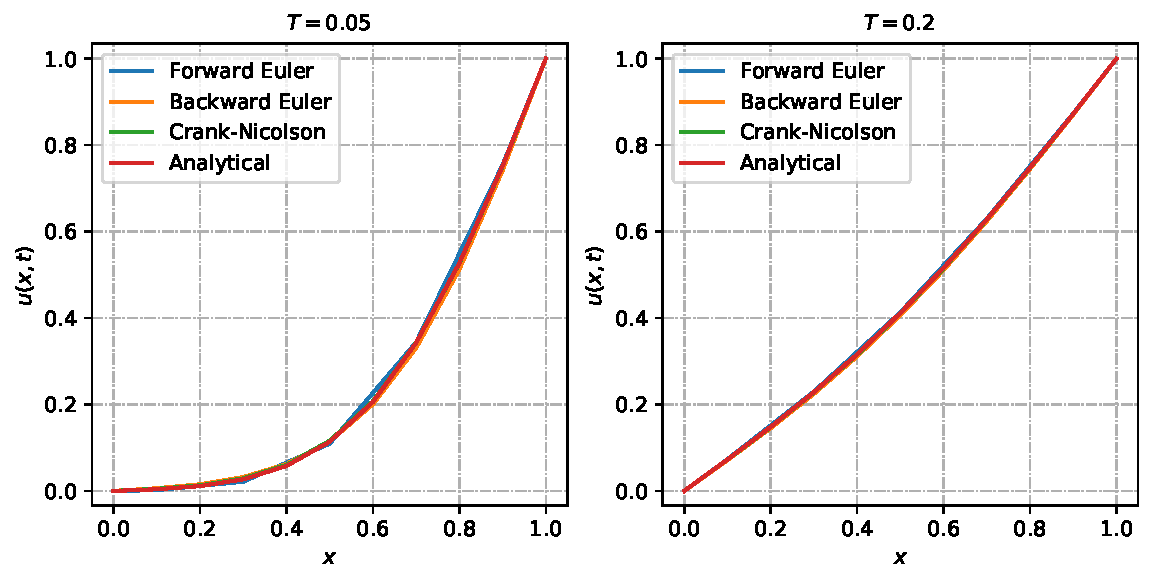
\includegraphics[scale=.6]{../Results/Comparison_1.pdf} 
        \caption{Comparison of solution for all three methods with CFS,  using $\Delta x=0.1$}
        \label{fig:Comparison1}   
\end{figure}  

\begin{figure}[!htb]
        \centering 
         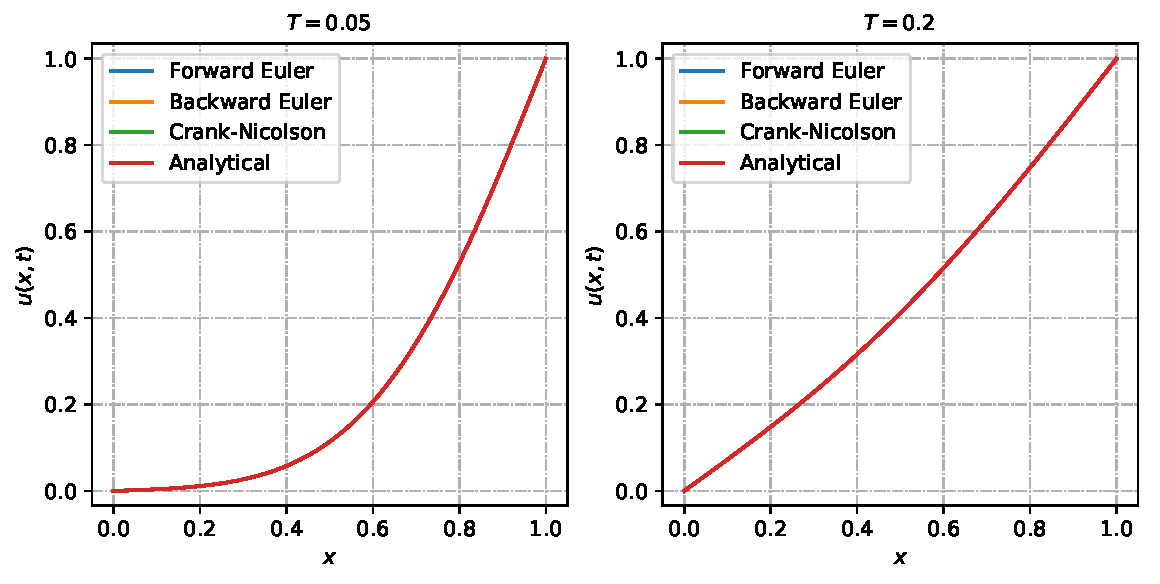
\includegraphics[scale=.6]{../Results/Comparison_2.pdf} 
        \caption{Comparison of solution for all three methods with CFS,  using $\Delta x=0.01$}
        \label{fig:Comparison2}   
\end{figure}  

\begin{table}
    \centering
    \caption{Maximum relative error}
\pgfplotstabletypeset[
column type=l,
every head row/.style={
before row={
\toprule &  \multicolumn{2}{c}{$\Delta x =0.1$} & \multicolumn{2}{c}{$\Delta x =0.01$}\\
},
after row=\midrule,
},
every last row/.style={
after row=\bottomrule},
columns/Method/.style ={column name=Method},
columns/t1/.style ={column name= { $  T=0.05$}},
columns/t2/.style={column name={ $  T=0.2$}},
columns/t3/.style={column name={ $  T=0.05$}},
columns/t4/.style={column name={ $  T=0.2$}},
col sep=&,row sep=\\,
string type,
]{
Method & t1 & t2 & t3 & t4 \\  
FW Euler&$5 \cdot 10^{-1}$ & $2.2 \cdot 10^{-2}$ & $5.1 \cdot 10^{-3}$ & $4.3 \cdot 10^{-4}$\\ 
BW Euler&$5.5 \cdot 10^{-1}$ & $2 \cdot 10^{-2}$ & $7.9 \cdot 10^{-3}$ & $2 \cdot 10^{-5}$\\ 
Crank-Nicolson&$2 \cdot 10^{-1}$ & $2.6 \cdot 10^{-3}$ & $2.5 \cdot 10^{-3}$ & $1.6 \cdot 10^{-4}$\\  }
\label{tab:MaxError1}
\end{table}



\begin{table}
    \centering
    \caption{Average relative error}
\pgfplotstabletypeset[
column type=l,
every head row/.style={
before row={
\toprule &  \multicolumn{2}{c}{$\Delta x =0.1$} & \multicolumn{2}{c}{$\Delta x =0.01$}\\
},
after row=\midrule,
},
every last row/.style={
after row=\bottomrule},
columns/Method/.style ={column name=Method},
columns/t1/.style ={column name= { $  T=0.05$}},
columns/t2/.style={column name={ $  T=0.2$}},
columns/t3/.style={column name={ $  T=0.05$}},
columns/t4/.style={column name={ $  T=0.2$}},
col sep=&,row sep=\\,
string type,
]{
Method & t1 & t2 & t3 & t4  \\  
FW Euler&$9.6 \cdot 10^{-2}$ & $6.5 \cdot 10^{-3}$ & $9.9 \cdot 10^{-4}$ & $1.8 \cdot 10^{-4}$\\ 
BW Euler&$1.2 \cdot 10^{-1}$ & $9.4 \cdot 10^{-3}$ & $1.9 \cdot 10^{-3}$ & $1.3 \cdot 10^{-5}$\\ 
Crank-Nicolson&$4.5 \cdot 10^{-2}$ & $1.3 \cdot 10^{-3}$ & $6.5 \cdot 10^{-4}$ & $8.5 \cdot 10^{-5}$\\  }
\label{tab:AvrError1}
\end{table}


\begin{figure}[!htb]
        \centering 
         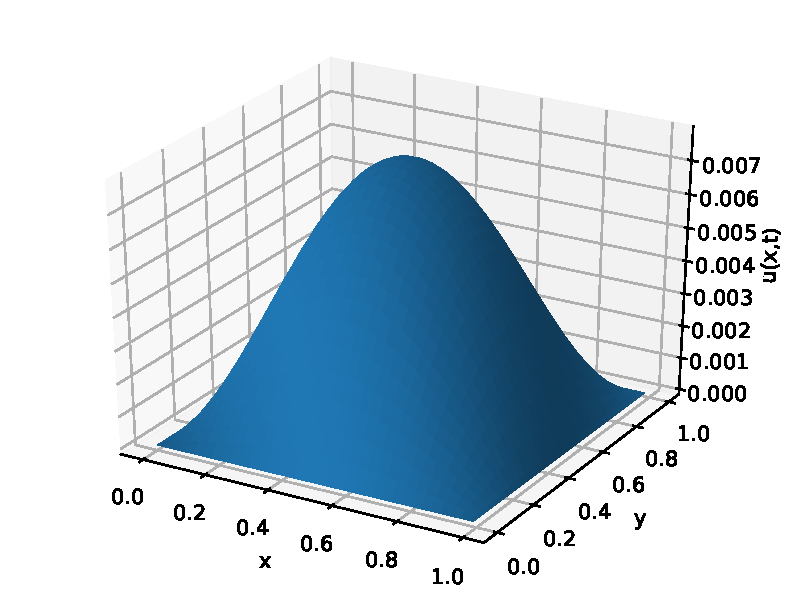
\includegraphics[scale=.7]{../Results/2dexact.pdf} 
        \caption{Plot of CFS using $h=0.01$, $\Delta t=\frac{1}{4} h^2$, and $T=0.2$}
        \label{fig:2dexact}   
\end{figure}  

\begin{figure}[!htb]
        \centering 
         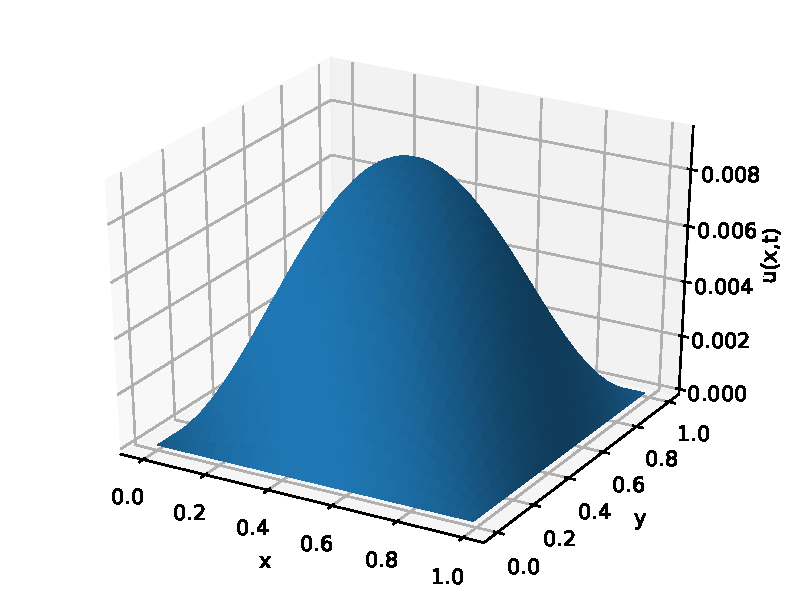
\includegraphics[scale=.7]{../Results/2dnumerical.pdf} 
        \caption{Plot of results from 2D explicit FW Euler using $h=0.01$, $\Delta t=\frac{1}{4} h^2$, and $T=0.2$}
        \label{fig:2dnumerical}   
\end{figure}  


\begin{figure}[!htb]
        \centering 
         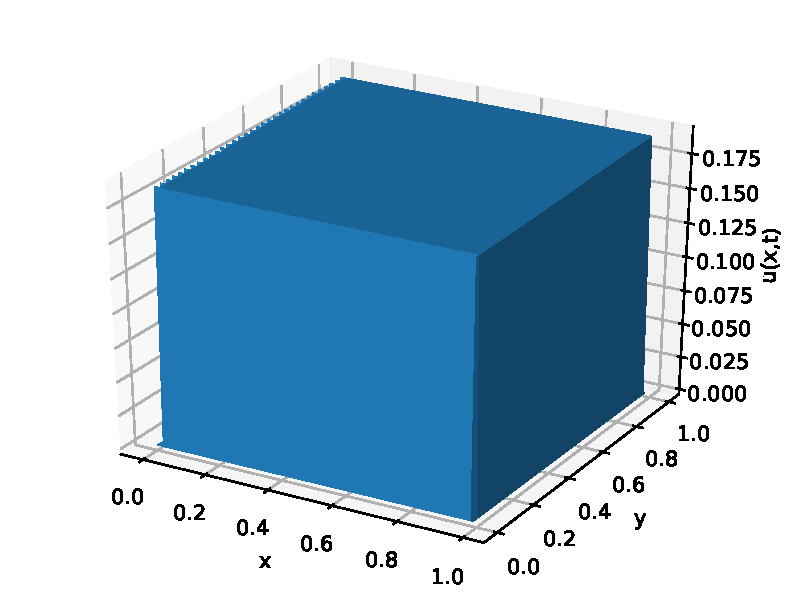
\includegraphics[scale=.7]{../Results/2drelerr.pdf} 
        \caption{Plot of relative error from 2D explicit FW Euler using $h=0.01$, $\Delta t=\frac{1}{4} h^2$, and $T=0.2$}
        \label{fig:2drelerr}   
\end{figure}  

\begin{table}[h!tb]
    \centering
    \caption{2DHQ: Average relative error when varying $\Delta t=\gamma h^2$}
\pgfplotstableset{% global config, for example in the preamble
% these columns/<colname>/.style={<options>} things define a style
% which applies to <colname> only.
columns/g/.style={fixed zerofill,precision=4,column name=\textsc{$\gamma $}},
columns/h1/.style={precision=6,column name=\textsc{$h=0.1 $}},
columns/h2/.style={precision=6,column name=\textsc{$h=0.01 $}},
columns/h3/.style={precision=6,column name=\textsc{$h=0.005 $}},
empty cells with={--}, % replace empty cells with ’--’
every head row/.style={before row=\toprule,after row=\midrule},
every last row/.style={after row=\bottomrule}
}
\pgfplotstabletypeset[ % local config, applies only for this table
1000 sep={\,},
columns/info/.style={sci zerofill
}
]
{rgamma.dat}
\label{tab:2DHQ.gamma}
\end{table}

\section{Discussion of results}
Figures \ref{fig:Comparison1} and \ref{fig:Comparison2} indicate that the initial implementation was successful, as the plots produced are similar to the CFS for all chosen parameters. In the $\Delta x=0.1$, the explicit FW and implicit BW Euler schemes have visually detectable deviations from CFS. This is however to be expected, as $\Delta x$ is quite small. \newline
Table \ref{tab:AvrError1}, shows the average relative error (ARE) for all three methods, for both $\Delta x=0.1$ and $\Delta x=0.01$ in the $T=0.05$ (referred to curved $u$) and $T=0.2$ (referred to as linear $u$) cases. A cursory examination indicate that most of the displayed relative errors as functions of $\Delta x$ are within the expected magnitudes, the exceptions being the curved $u$, $\Delta x=0.1$ case, and for the explicit and implicit Euler schemes also in the linear $u$, $\Delta x=0.1$ case. This may either indicate implementation error or wrongly expected precision. A possible reason may be that the parameters do not allow the numerical solutions a sufficient number of cycles with respect to $\Delta t$ vs $T$. As the table shows average values, it may be that the methods mostly produce results within the expected error magnitudes, and that the average error is significantly shifted due to outliers at critical values of $x$. All inn all, the error magnitude appears to be $10^{-2}$ to $10^{-3}2$ for $\Delta x=0.1$ with the exception of BW Euler ($10^{-1}$ for curved $u$), and in the $\Delta x=0.01$ case, between $10^{-3}$ to $10^{-5}$ for all methods. Both magnitude ranges are $\sim (\Delta x)^2$ and to a varying degree  $\sim \Delta t (\Delta x)^2$.  Further study of the relative error is divided into two separate cases, $\Delta x=0.1$ and $\Delta x=0.01$.\newline
\paragraph{1.}
In the $\Delta x=0.1$ case, the Crank-Nicolson scheme performs significantly better than the other two methods. indicating that this method is more suited when $\Delta x$ is relatively small. The maximum relative errors (MRE) in table \ref{tab:MaxError1} further bolsters this hypothesis, as the CN scheme has the lowest values in the $\Delta x=0.1$ case there as well. Looking at MRE, the FW and BW Euler methods appear to perform equally well. Comparison with ARE however, shows that the BW Euler falls behind the FW Euler in precision for low $\Delta x$. This may, again, be the result of outliers at critical points, but holds true with regards to relative error nonetheless. Based on this, the CN scheme appears to be the best suited for low $\Delta x$ (ARE $10^{-2}$ to $10^{-3}$), and the BW Euler the least suited (ARE curved $u$ one order of magnitude larger than CN) . 
\paragraph{2.}
Examination of the $\Delta x=0.01$ case shows a different trend than what is to be observed in the $\Delta x=0.1$ case. In terms of MRE, all three methods are within the same order of magnitude in the curved $u$ case, with the CN scheme performing the best. Comparing this to the corresponding ARE values, shows the same trend, with the exception of BW performing less well yet again. This, together with the earlier indications on BW Euler, indicates that BW Euler is unstuited for curved $u$ (error one order of magnitude larger than best method). Looking at the values for $T=0.2$, both ARE and MRE show that the FW Euler method falls behind in accuracy. This indicates a (relative) unsuitability for the method in cases where $\Delta t$ is high and $u$ linear. For linear $u$, BW Euler performs the best, closely followed by CN. This indicates that the BW Euler and CN schemes are well suited for curved $u$ and high $\Delta x$ (error $\sim 10^{-5}$. \newline
\paragraph{Remarks:}
The indications described above may be erroneous on account of implementation methods. In particular, the overall (relatively) poor performance by BW Euler leads to the possibility that discrepancies were made in either the algorithm or it's implementation.\newline

\paragraph{2 spatial dimentions:}
By visually comparing figures \ref{fig:2dexact} and \ref{fig:2dnumerical}, the implementation of the explicit FW Euler method to the 2D heat equation problem appears successful - both figures show solutions of the same shape and with the same order of magnitude for $h=0.01$, $\Delta t=\frac{1}{4} h^2$ at $T=0.2$. Table \ref{tab:2DHQ.gamma} (NaN - exceedingly large number), shows the average relative error (ARE) as a function of $\Delta t/h^2 = \gamma $, for various values of $h$. $\frac{\Delta t}{(\Delta x)^2}\leq \gamma=4$ appears to be the stability limit of the 2 dimensional explicit forward Euler scheme. For $h=0.1$ the ARE reaches reasonable values at $\gamma\approx 0.27$, but in both the $h=0.01$ and $h=0.005$ cases, $\gamma>1/4$ produce exceedingly large errors. When comparing the values of $h$ for $\gamma=1/4$, the error is reduced from $h=0.1$ to $h=0.01$, as is expected. However, the ARE is not even remotely close to $\sim h^2$. Additionally, the ARE appears to be approximately the same for $h=0.01$ and $h=0.005$. This may be due to a faulty algorithm, erroneous implementation, a wrongly calculated exact solution (either when derived  or implemented), average shift due to solution outliers, or due to the indication from the 1D case for the FW Euler to be unsuited for the choice of $T$. However, examining \ref{fig:2drelerr}, it is clear that the relative error approximately $0.175$ uniformly across the grid, which means that there are no outliers shifting the ARE.


\subsection{Conclusions}
Based on the indications described under discussion of results, it is concluded that overall error magnitudes are $\sim (\Delta x)^2$ and to a varying degree  $\sim \Delta t (\Delta x)^2$. The Crank-Nicolson scheme (local truncation error $\sim O((\Delta t)^2)$ and $O((\Delta x)^2)$) is concluded as the overall most precise method due to relative errors $\sim (\Delta x)^2$. In the case of solutions at low ratio of characteristic diffusive time, the implicit backward Euler scheme is concluded as the least suited. due to producing average relative errors one order of magnitude larger than the Crank-Nicolson method. On the other hand, for solutions closer to characteristic diffusion time, with a high number of discretization points, the implicit backward Euler scheme produced the smallest average relative errors ($1.3 \cdot 10^{-5}$). The explicit forward Euler method is concluded as unsuited for solutions at ratios to characteristic diffusion time higher than $\sim 0.1$ when large spatial grids are deployed. In the case of two spatial dimensions, the explicit forward Euler produces a solution similar to the closed form solution. No further conclusions may however be drawn on the 2 dimensional case, as discrepancies manifesting in the relative error not following the predicted local truncation error were observed. Lastly, it is possible that the code implementing the implicit backward Euler (in the 1D case) is erroneous. In order to verify the conclusions on this method, a re-examination of this method is therefore required.
\newline




\bibliography{ref}
\bibliographystyle{plain}


\end{document}





% ------------------- end of main content ---------------



